% Originally: content/week-03.tex, the Lipschitz block inside \subsection{Why do we care about compactness?}

\section{Lipschitz continuity}
\label{sec:lipschitz_continuity}

% Quelle: Linus Lüchinger/Slides/Slides-03-02.pdf, pp. 10--13 -- Sonnet 5 (Medium)
% Lüchinger's exercise slides motivate and name the condition and give a quick self-test; both
% are reproduced here, reformulated, since they fill a genuine gap in Corsin's own notes.
\begin{ainote}
The course never formally introduces Lipschitz continuity, even though a Lipschitz constant is
already used informally for contraction mappings (\cref{def:contraction_mapping}, below). The
definition and the hierarchy below are therefore supplied here, and will not be found under this
name in the lecture material.
\end{ainote}

\begin{definition}[Lipschitz continuity]
\label{def:lipschitz_continuous}
Let $(X,d_X)$, $(Y,d_Y)$ be metric spaces. A function $f : X \to Y$ is \newterm{Lipschitz
continuous} (\germanterm{Lipschitz-stetig}) if there exists $L \geq 0$, a \newterm{Lipschitz
constant} for $f$, such that
\[d_Y(f(x),f(x')) \leq L\cdot d_X(x,x') \quad \text{for all } x,x' \in X.\]
\end{definition}

\begin{remark}[Hierarchy of continuity notions]
\label{rem:continuity_hierarchy}
Lipschitz continuity is stronger than uniform continuity
(\cref{def:uniformly_continuous}), which in turn is stronger than continuity
(\cref{def:continuous}). For the first implication, assume $L > 0$ (for $L = 0$ the function is
constant and there is nothing to prove); then $\delta := \varepsilon/L$ satisfies the definition
of uniform continuity, since
\[d_X(x,x') < \frac{\varepsilon}{L} \quad \text{gives} \quad d_Y(f(x),f(x')) \leq L\,d_X(x,x') < \varepsilon\]
for \emph{every} pair $x,x'$. This is one and the same $\delta$ at every point, which is exactly
what uniform continuity asks for. The second implication is immediate: a $\delta$ that works at
all points in particular works at each one.

Both converses fail. Every continuously differentiable function on a compact \emph{interval} is
Lipschitz continuous, with $L := \sup|f'|$ by the mean value theorem. The word \emph{interval}
matters here, since the mean value theorem needs the segment between the two points to lie in the
domain. But $f(x) := \sqrt{x}$ on $[0,\infty)$ is uniformly continuous and \emph{not} Lipschitz.
A Lipschitz constant would force $\delta$ to shrink only linearly in $\varepsilon$, whereas here
$|\sqrt{x}-\sqrt{x'}| < \varepsilon$ near $0$ already requires $\delta$ of order
$\varepsilon^2$. The reason is visible in the graph, since the tangent at $0$ is vertical and no
finite slope $L$ can dominate it.
\end{remark}

% Sonnet 5 (Medium)
\begin{center}
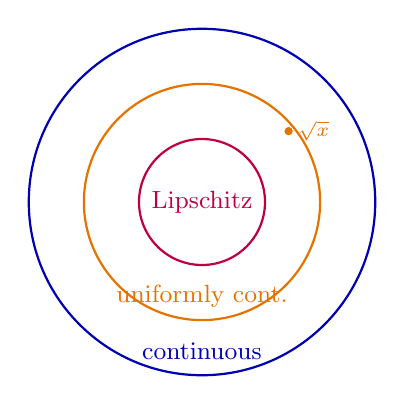
\begin{tikzpicture}[scale=1.0]
  \draw[blue!70!black, thick] (0,0) circle (2.2);
  \node[blue!70!black, font=\small] at (0,-1.9) {continuous};
  \draw[orange!90!black, thick] (0,0) circle (1.5);
  \node[orange!90!black, font=\small] at (0,-1.2) {uniformly cont.};
  \draw[purple, thick] (0,0) circle (0.8);
  \node[purple, font=\small] at (0,0) {Lipschitz};
  \fill[orange!90!black] (1.1,0.9) circle (1.5pt) node[right, font=\scriptsize] {$\sqrt{x}$};
\end{tikzpicture}
\end{center}

% Supplement: Linus Lüchinger/Slides/Slides-03-02.pdf, slide 13
% Was an `aiexercise` labelled ex:ai_continuity_classification. It is Linus's exercise, not
% one invented here, so by the ai*-prefix rule it is a plain `exercise` with a provenance
% comment; only the solution below is authored. His domain for the first row was [0.5,1];
% widened to [0,infty) so that the row separates uniform continuity from Lipschitz, which is
% the distinction \cref{rem:continuity_hierarchy} has just drawn.
\begin{exercise}[Classifying continuity]
\label{ex:continuity_classification}
For each of the following functions, determine whether it is continuous, uniformly continuous,
and/or Lipschitz continuous on the given domain:
\begin{center}
\begin{tabular}{ll}
\textbf{Function} & \textbf{Domain} \\
\hline
$\sqrt{x}$ & $[0,\infty)$ \\
$1/x$ & $(0,1)$ \\
$\sgn(x)$ & $(-1,1)$ \\
$|x|^{3/2}$ & $(-1,1)$
\end{tabular}
\end{center}
\end{exercise}


% --- exercises relocated here from the dissolved sheet 3 ---

% Originally: content/exercise-sheets/week-03.tex, problem 3.1
% Source: exercises/Ex3_Analysis2_eng.pdf

\begin{exercise}[3.1 --- Lipschitz or not]
\label{ex:3.1}
Give an example of:
\begin{enumerate}[label=\textbf{(\alph*)}]
  \item A $\tfrac{1}{2}$-Lipschitz function $f : [0,1) \to [0,1)$ that has no fixed point.
  \item A map $f : \mathbb{R}^2 \to \mathbb{R}^2$ that has no fixed point, but is an isometry,
    i.e.\ $\|f(x) - f(x')\| = \|x - x'\|$ for all $x, x' \in \mathbb{R}^2$.
\end{enumerate}
\end{exercise}

% Originally: content/exercise-sheets/week-03.tex, problem 3.6
% Source: exercises/Ex3_Analysis2_eng.pdf

\begin{exercise}[3.6 --- Multiple choice (uniform continuity)]
\label{ex:3.6}
Select all the statements below that are true.
\begin{enumerate}[label=\textbf{(\alph*)}]
  \item The function $(x,y) \mapsto x+y$ is uniformly continuous in $\mathbb{R}^2$.
  \item The function $(x,y) \mapsto xy$ is uniformly continuous in $\mathbb{R}^2$.
  \item The function $(x,y) \mapsto x+y$ is uniformly continuous in $[0,1]^2$.
  \item The function $(x,y) \mapsto xy$ is uniformly continuous in $[0,1]^2$.
\end{enumerate}
\end{exercise}

\begin{remark}
Corsin's third reason to care about compactness (\cref{sec:why_compactness_matters}) is precisely
that a continuous function on a compact space is uniformly continuous, which settles
\cref{ex:3.6}(c) and (d) at once.
\end{remark}

% Originally: content/exercise-sheets/week-03.tex, problem 3.11
% Source: exercises/Ex3_Analysis2_eng.pdf

\begin{exercise}[3.11 --- (*) Uniform continuity and moduli of continuity]
\label{ex:3.11}
Let $(X,d_X)$ and $(Y,d_Y)$ be metric spaces and let $f : X \to Y$.

A \textbf{modulus of continuity} is a function $\omega : [0,\infty) \to [0,\infty]$ such that
$$\omega(0) = 0, \qquad \omega \text{ is nondecreasing}, \qquad \lim_{t \downarrow 0}\omega(t) = 0.$$
(Here $[0,\infty]$ means we also allow the value $+\infty$.) We say that $f$ \textbf{has modulus
of continuity} $\omega$ if
$$d_Y\big(f(x), f(y)\big) \leq \omega\big(d_X(x,y)\big) \qquad \forall x,y \in X.$$
\begin{enumerate}[label=\textbf{\arabic*.}]
  \item Prove that $f$ is uniformly continuous on $X$ if and only if $f$ has a modulus of
    continuity.
  \item \textit{(Bonus 1)} Assume $X \subset \mathbb{R}$ is an interval with the usual distance
    $d_X(x,y) = |x-y|$. Show that the modulus constructed in (1) can be chosen
    \textbf{subadditive}, i.e.\ $\omega(t_1+t_2) \leq \omega(t_1) + \omega(t_2)$ for all
    $t_1, t_2 \geq 0$.
  \item \textit{(Bonus 2)} Assume $X \subset \mathbb{R}^n$ is \textbf{convex}, meaning: for all
    $x_1, x_2 \in X$ and all $\lambda \in [0,1]$, $(1-\lambda)x_1 + \lambda x_2 \in X$. With
    $d_X(x,y) = \|x-y\|$ (Euclidean distance), show again that the modulus from (1) can be chosen
    subadditive.
\end{enumerate}

\begin{remark}[official]
In general metric spaces a modulus of continuity may have infinite value for finite $t > 0$.
Example: $X = \mathbb{Z}$ with the usual distance, $Y = \mathbb{R}$, $f(n) = n^2$. This $f$ is
uniformly continuous on $\mathbb{Z}$ (because points closer than 1 must be equal), but no finite
$\omega(1)$ can bound $|f(n+1) - f(n)| = 2n+1$ for all $n$. Allowing the value $+\infty$ avoids
this issue, and in many familiar settings (e.g.\ intervals/convex sets in $\mathbb{R}^n$) the
resulting $\omega_f(t)$ is finite for all $t$.
\end{remark}

\textit{Official hints:} \textbf{3.11.1:} define the ``worst oscillation at scale $t$''
$\omega_f(t) := \sup\{d_Y(f(x),f(y)) : d_X(x,y) \leq t\}$. \textbf{3.11.2 / 3.11.3:} if
$d_X(x,y) \leq t_1 + t_2$, choose an intermediate point $z$ on the segment from $x$ to $y$ so
that $d_X(x,z) \leq t_1$ and $d_X(z,y) \leq t_2$, then use the triangle inequality in $Y$.
\end{exercise}
